\chapter{User study}
\label{sec:user_study_chapter}
%
% USER STUDY CHAPTER
%

From August 21th to September 12th 2017, I conducted a user study that aimed at gathering data to compare with the results of processing 3D objects according to \textit{mesh saliency} \cite{lee2005mesh}. However, due to the fact that the projection installation at the V2C was not available for me at all times, I could not use every day in that timespan. The installation was assigned to me for a total seven days. I was able to collect a reasonable amount of data from a sufficiently sized group of participants. This chapter will go over details of how I organised and conducted the user study.

As briefly described before in section \ref{sec:conduct_user_study_with_the_selection_application}, I asked participants to use my selection application and the hardware available at the V2C to select regions of 3D objects they found \textit{interesting}. In general, participants got familiar with the devices and interaction mechanics quickly and were able to make selections according to their perception of what was of importance.
% @TODO: Kurzen Spoiler einbauen, wie es sich mit den Unterschieden verhalten hat (das Ziel der ganzen verf*ckten Arbeit halt)

\section{Hardware used}
\label{hardware_used}
%
% HARDWARE USED
%

The five-sided projection installation at the V2C is equipped with several devices which can be tracked inside of it. Users taking part in the user study were asked to put on a pair of lightweight stereoscopic glasses, shown in figure \ref{fig:glasses}. Note the three white, spherical parts on each side of the glasses. These are used for tracking their position, orientation, tilt and yaw within the projection installation. According to these parameters, two images are projected onto the walls of the installation from behind, each for one eye. The glasses are in synchronisation with the projectors and actively switch between left and right 120 times per second, only showing one of the projected images at a time. This way, an immersive 3D effect for one user wearing the glasses within the installation is created.  

\begin{figure}[htb]
  \centering
  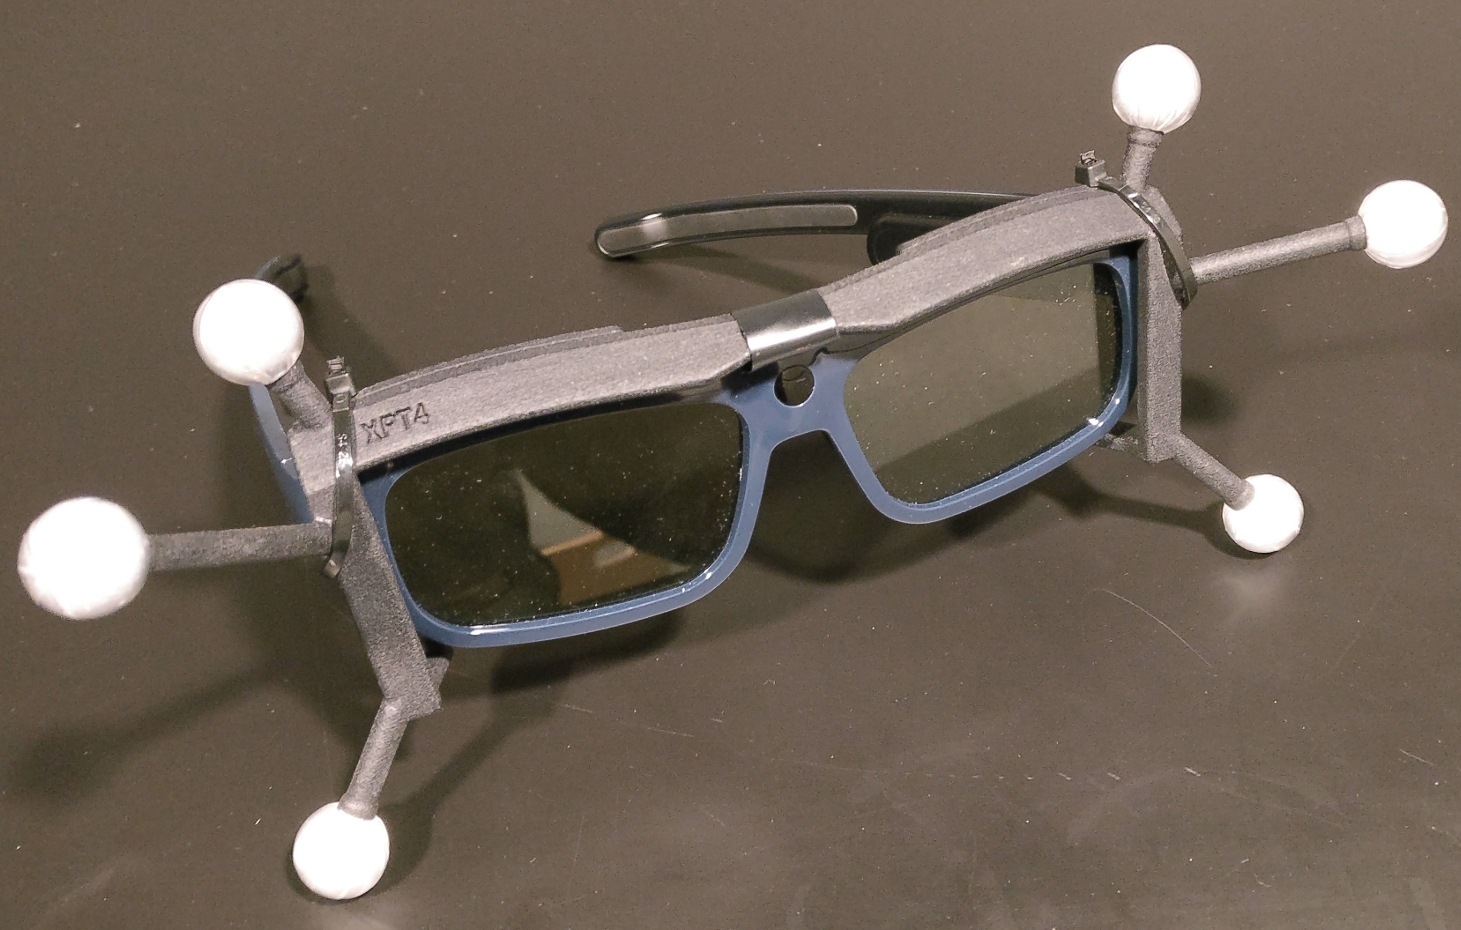
\includegraphics[width=.8\textwidth]{concept_glasses.jpg}\\ % PNG-File
  \caption{The trackable, stereoscopic glasses used at the V2C}\label{fig:glasses}
\end{figure}

For interaction, a handheld device called \textit{wand} see figure \ref{fig:wand}, is used within the projection installation. It allows for navigation within the scene via a little joystick as well as interaction with four buttons. The joystick moves the scene in the opposite way the user pushes it. This has been described as counter-intuitive by some users.

As described in \ref{sec:selection_process}, two of those buttons are enough for the selection application's needs. The button on top of the \textit{wand}, on the left side of the joystick is used for making selections on the currently loaded 3D object, the button  right to it can be used to clear already marked selections. Figure \ref{fig:wand} shows the device. Again, note the white, spherical parts used for tracking position, orientation, tild and yaw of the device attached to it.

\begin{figure}[htb]
  \centering
  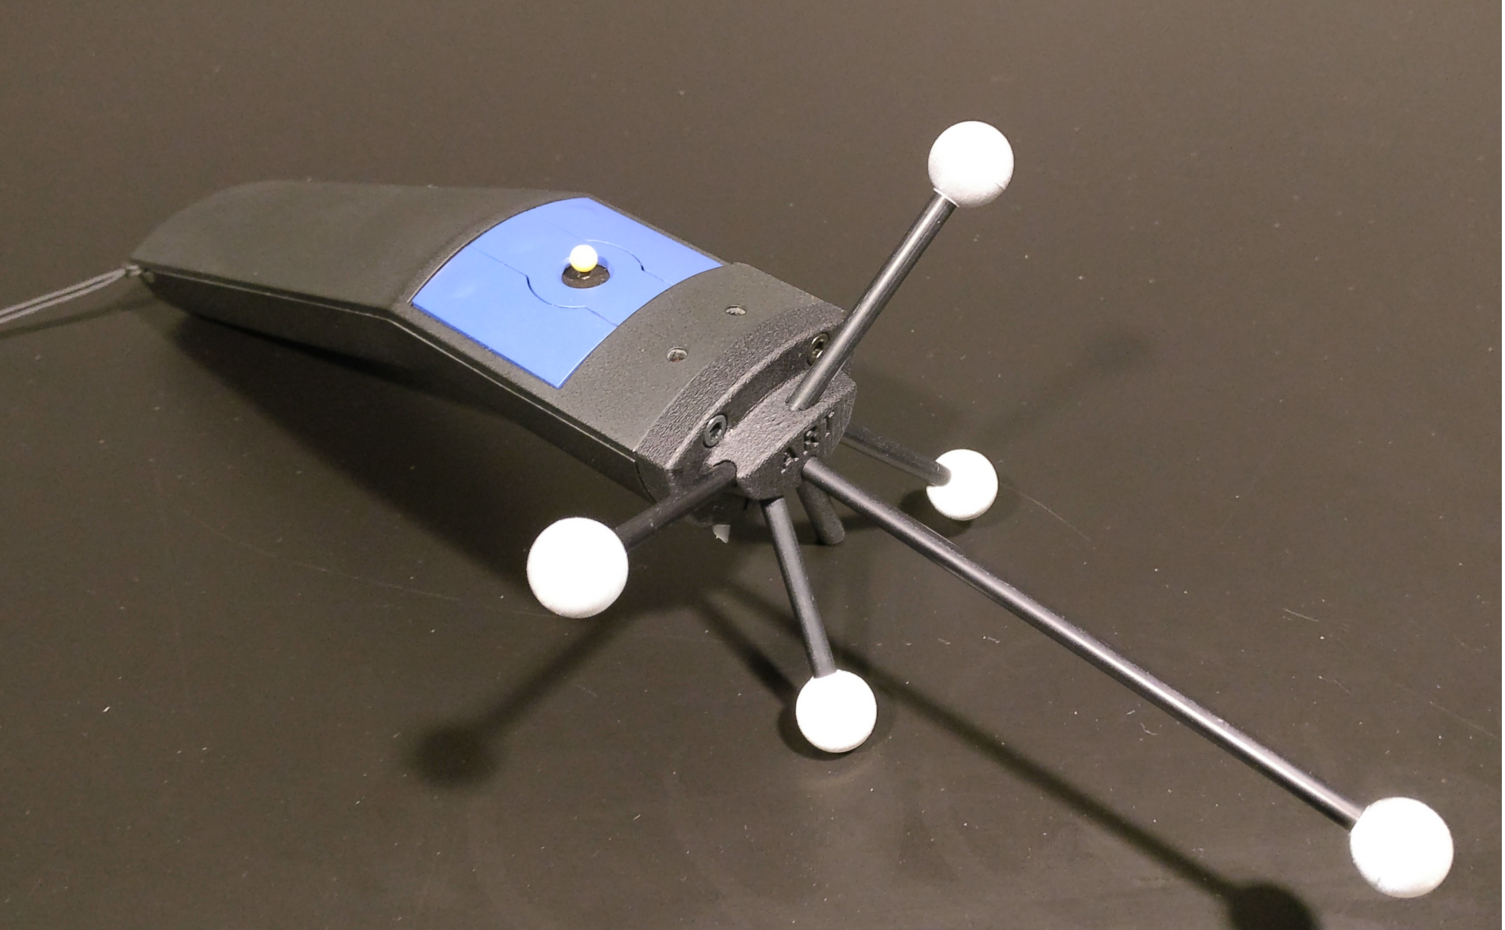
\includegraphics[width=.8\textwidth]{concept_wand.jpg}\\ % PNG-File
  \caption{The input device used at the V2C}\label{fig:wand}
\end{figure}

% @TODO: (Reminder, siehe 03-concept, hier darauf verweisen oder umgekehrt)
% @TODO: Bild rausrendern (user mit Wand in der Hand, geladenem Object + wand_pos), schneiden und uploaden


\section{Models used}
\label{models_used}
%
% MODELS USED
%

Regarding objects used for the study, I aimed at offering as much variety of types of objects among as few objects as possible. The motivation for this was to achieve results that are genereally applicable for any type of geometric data, at least to an basic extent. Also, to avoid the users losing motivation due to repeating tasks during the study, keeping the number of objects to a minimum was a constraint to be considered.
I decided to use three objects described table in \ref{tab:userstudy_objects} and depicted in figure \ref{fig:all_objects}.

\begin{table}[]
\centering
	\begin{tabular}{l|l|l|l|l}
		object	& created through	& source	& vertex count	& class of objects	\\ \hline
		cow	& 3D modelling		& \cite{cow}	& 69,648	& purely natural	\\
		P51 Mustang	&	3D modelling	& \cite{P51}	& 51,708	& purely mechanical	\\
		bunny sculpture	&	3D scan	& \cite{bun}	& 68,754	& natural, man-made	
	\end{tabular}
	\caption{3D objects used in the study}
	\label{tab:userstudy_objects}
\end{table}
% table 3.1

Note that the models are from third-party vendors. I made sure they are all free to use for educational purposes and weblinks to where they have been published originally are provided in the bibliography.

\begin{figure}[htb]
  \centering
  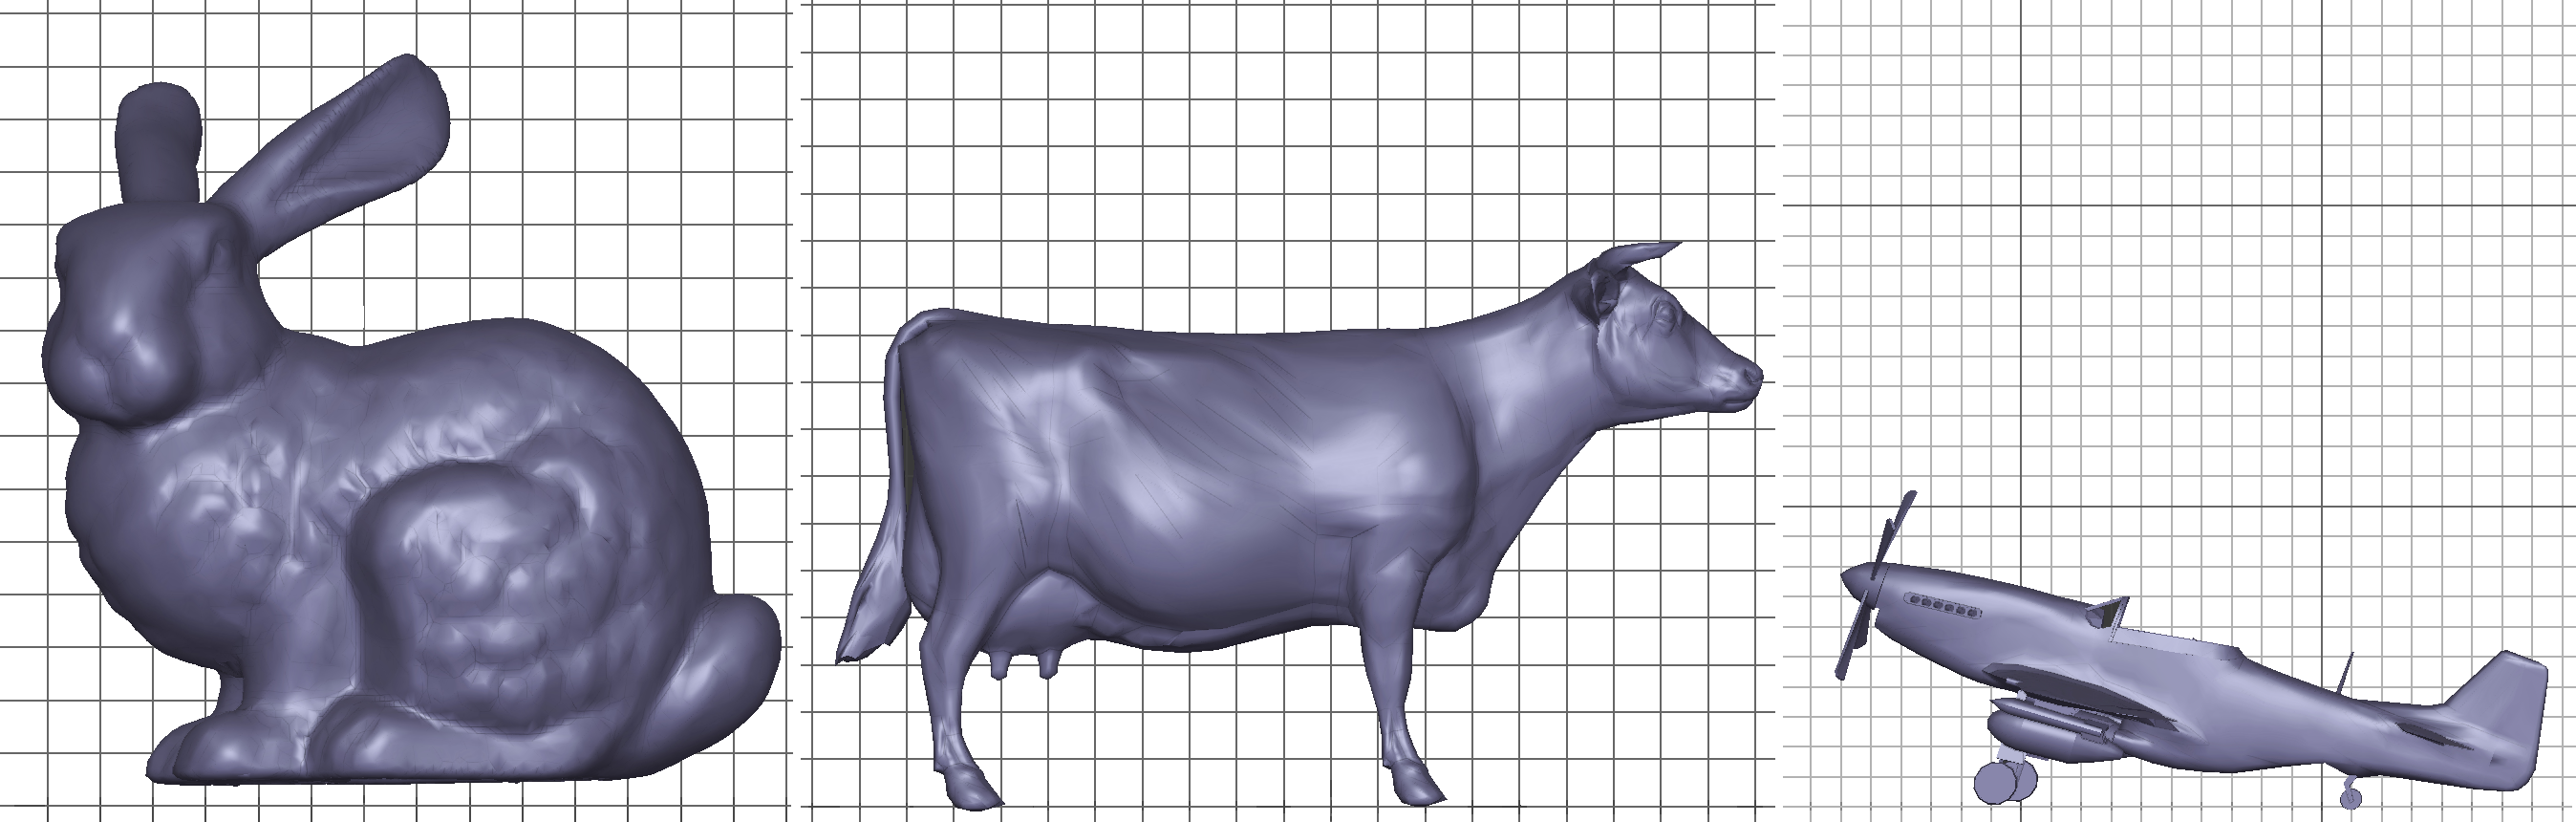
\includegraphics[width=1.0\textwidth]{userstudy_all_objects.png}\\ % PNG-File
  \caption{The 3D objects used for the user study}\label{fig:all_objects}
\end{figure}

Figure \ref{fig:all_objects} shows the objects used in the user study. From left to right, the 3D scanned bunny, the modelled cow and the low-poly, modelled aircraft are shown. Consider the grid to get a sense of their proportions. I did not scale them according to their real world sizes and instead made them take up approximately equal space in the virtual scene. This was done with the intention to provide a similar level of visual detail, independent of the actual geometric level of detail, for each object. Furthermore, I wanted to prevent the size of the objects from having any sort of influence on how users perceived them.


\section{Tasks given}
\label{tasks_given}
%
% TAKS GIVEN
%

Users were asked to use the hard- and software available to select regions and parts of the objects they deemed \textit{interesting} since \textit{mesh saliency} claims to be able to reliably predict such parts \cite{lee2005mesh}. I told the users that this would be the task at hand only after they stated they felt ready to interact with the scene presented in the projection installation. They were given as much time as they wanted to get somewhat accustomed to navigating and the selection process it but in general, nobody took longer than a few minutes.

I then explained the course of the user study, going over the following instructions:
\begin{itemize}
	\item The task is to select parts and regions of the objects users consider \textit{important}.
	\item Some suggestions as to what could be considered \textit{important}:
		\begin{itemize}
			\item \textit{what do you consider visually interesting or important?}
			\item \textit{what do you assume are natural focus points of attention?}
			\item \textit{what parts do you consider vital for identifying the object?}
		\end{itemize}
	\item However these are just ideas, in general users were encouraged to select whatever they, personally, deemed \textit{important} according to their own understanding. I made sure to emphasise this because I aimed for natural results.
	\item There is no \textit{correct} way to make the selection. Users were, again, encouraged to make selection according to their perception.
	\item How precise the selections would be was up to users. If they were satisfied, that was the desired level of precision
	\item I asked to consider symmetry to some extent in the selection where possible.
	\item The time limit per object was five minutes. I made clear that the selection process would be stopped after that period of time.
	\item However, if users would be satisfied with the selection earlier, I encouraged them to say so. In this case, if there were still objects left to work with, the next one would be presented. Otherwise, the practical part of the user study was finished.
\end{itemize}

 

\section{Shortcomings of the study design}
\label{shortcomings_of_the_study_design}
While conducting the user study, I noticed some factors which possibly had negative impacts on the outcome of it. On top of that, a few technical issues emerged which could have made the experience for the users less immersive and convincing. I will go over all these issues in the following subsections. I cannot describe the extent they influenced the study, this is solely meant to document them.

\subsection{Task, instructions and questions}
\label{task_instructions_questions}
%



\subsection{Technical issues}
\label{technical_issues}
%
% TECHNICAL ISSUES
%

% ab 05.09.207 ist ein Projektor ausgefallen
% Projektor "oben" hatte höhere Framerate
% Gelegentliche Abstürze bei zu schnellen Bewegungen
% Tracking Probleme



\section{Participant demographics}
\label{participant_demographics}
